% Figure 1: Task schematic
\begin{figure}[htbp]
\centering
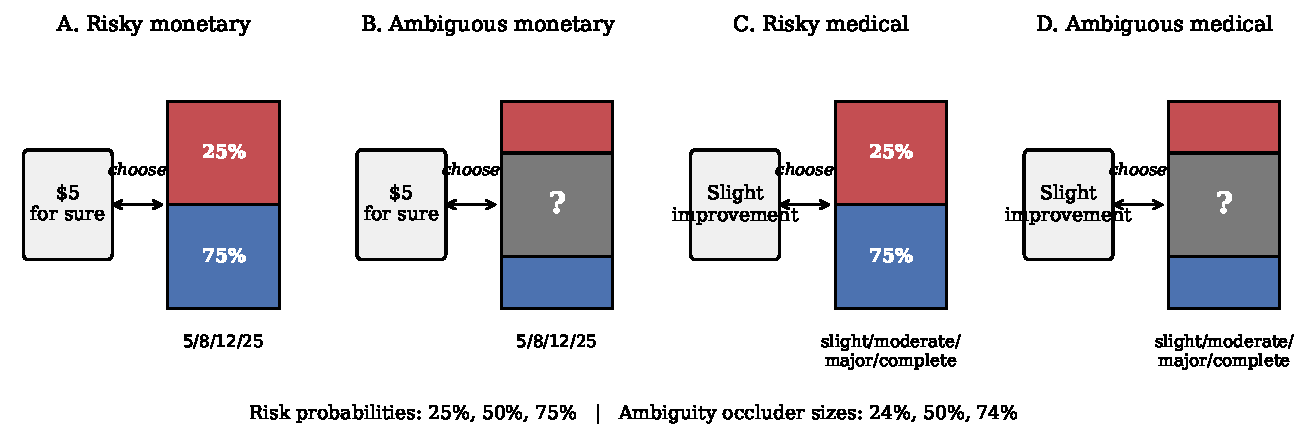
\includegraphics[width=\textwidth]{figures/fig1_task_schematic.pdf}
\caption{Task design. On every trial participants choose between a certain option (left) and an uncertain lottery (right). In risky trials (A, C) outcome probabilities are fully disclosed by red and blue bar proportions; in ambiguous trials (B, D) the centre of the bag is occluded by a grey rectangle, leaving the probability only partially known. Outcome probabilities in risky trials were 25\%, 50\% and 75\%; occluder sizes in ambiguous trials were 24\%, 50\% and 74\%. Monetary outcomes on the right side were \$5, \$8, \$12 and \$25; medical outcomes were slight, moderate, major and complete recovery, paired with a certain option of \$5 or ``slight improvement'' respectively.}
\label{fig:task}
\end{figure}

% Figure 2: Estimated added subjective values
\begin{figure}[htbp]
\centering
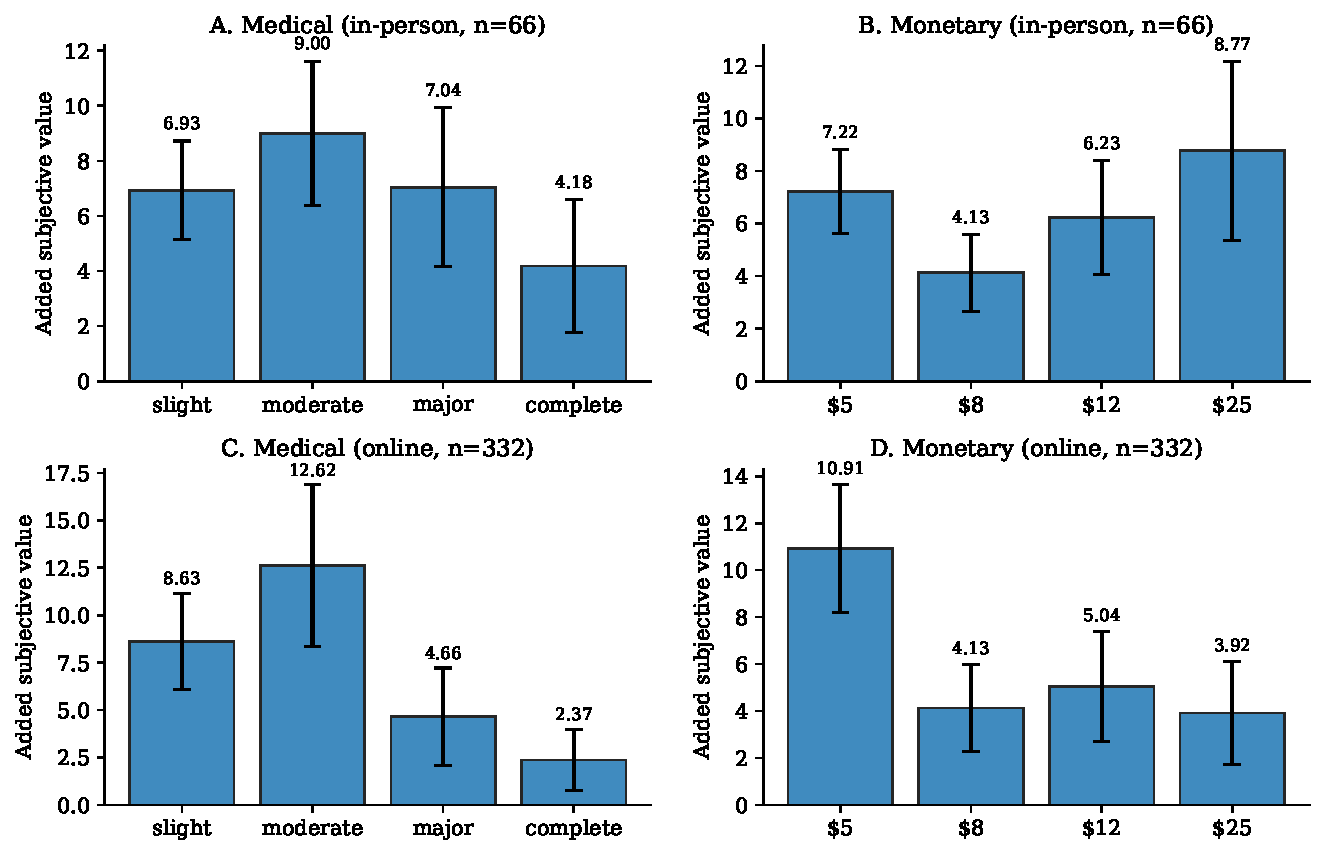
\includegraphics[width=0.95\textwidth]{figures/fig2_estimated_values.pdf}
\caption{Added subjective values extracted by the Estimated Value model. Each bar is the posterior mean of the added value for the corresponding outcome category (increment relative to the preceding category), with error bars showing one standard deviation across participants. Panels A and C show medical outcomes, panels B and D show monetary outcomes; top row is the in-person sample ($n=66$) and bottom row the online sample ($n=332$).}
\label{fig:values}
\end{figure}

% Figure 3: Cross-domain association
\begin{figure}[htbp]
\centering
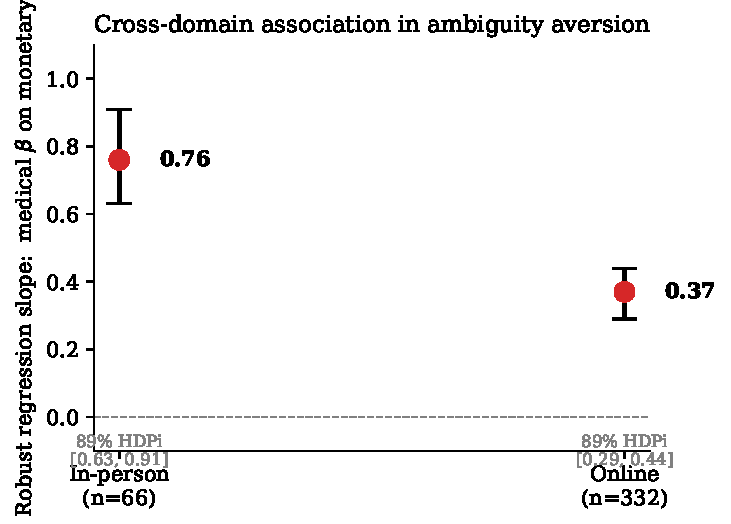
\includegraphics[width=0.65\textwidth]{figures/fig3_cross_domain.pdf}
\caption{Cross-domain association in ambiguity aversion ($\beta$). Points show the posterior mean slope of a robust regression of medical $\beta$ on monetary $\beta$; error bars show the 89\% highest density posterior interval. The association is strongly positive in both the in-person sample (slope = 0.76, 89\% HDPi [0.63, 0.91]) and the online sample (slope = 0.37, 89\% HDPi [0.29, 0.44]), indicating that ambiguity aversion is a trait that generalises across decision domains.}
\label{fig:cross}
\end{figure}

% Figure 4: Simulation grid
\begin{figure}[htbp]
\centering
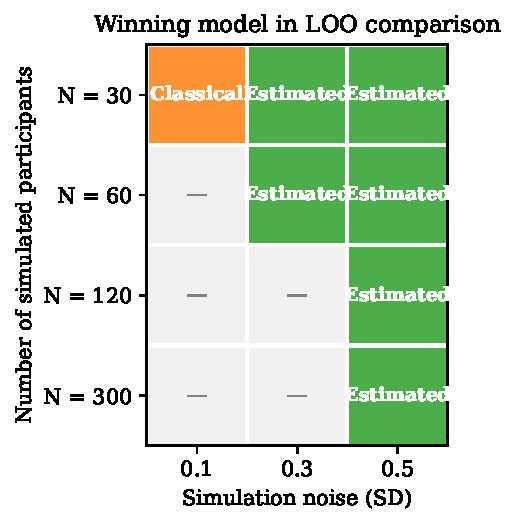
\includegraphics[width=0.65\textwidth]{figures/fig4_simulations.pdf}
\caption{Simulation results. Each coloured cell is a simulated participant group characterised by its sample size $N$ and the standard deviation of Gaussian noise injected on the generative $\alpha$ and $\beta$ parameters. The cell colour indicates which model achieves higher LOO: the Classical Utility model wins only at the lowest noise level (SD = 0.1); at higher noise the Estimated Value model wins regardless of sample size. Grey cells were not tested in the extracted simulation grid.}
\label{fig:sims}
\end{figure}
